\chapter{Intrusive Diagnostics and Their Limitations}
\label{ch:probes}

The quantification of ion energy flux across a plasma sheath has historically been approached through diagnostics that place a solid object directly into the plasma and interpret the currents, voltages, or particle fluxes it collects. Electrostatic (Langmuir) probes, retarding-field energy analyzers, and their derivatives remain the most widely deployed tools for measuring electron temperature, plasma density, plasma potential, and ion energy distributions. Their appeal is clear: inexpensive, mechanically simple, high-resolution, and grounded in a century-old analytic theory. Yet every intrusive probe measurement is, by construction, a measurement of a plasma locally modified by the probe itself: it nucleates its own sheath, draws a compensating return current, and in high-flux or magnetized environments may not survive the flux it is meant to quantify. This chapter develops the theory of electrostatic probe diagnostics, catalogs the principal probe geometries, and then turns critically to three limitations motivating the non-intrusive alternatives pursued later: perturbation from probe-sheath formation, physical degradation in high-flux environments, and interpretive ambiguities in non-Maxwellian or magnetized plasmas.

\section{Langmuir Probe Theory}
\label{sec:probes-langmuir-theory}

\subsection{Historical Basis and the Collected Current}

The electrostatic probe technique originates with Langmuir's analysis of the current collected by a small biased electrode in a low-temperature discharge, and remains the most direct method for extracting local electron density, temperature, and plasma potential; refined slope-extraction procedures continue to convert Langmuir's original graphical method into forms suitable for automated data reduction \cite{ref0217}.

A probe of collecting area $A_{\mathrm{p}}$ immersed in a plasma and biased to a voltage $V$ relative to a fixed reference collects a net current
\begin{equation}
I(V) = I_{\mathrm{e}}(V) - I_{\mathrm{i}}(V),
\label{eq:probe-net-current}
\end{equation}
where $I_{\mathrm{i}}(V)$ and $I_{\mathrm{e}}(V)$ are the ion and electron currents at that bias, positive net current corresponding to net electron collection. Sweeping $V$ across several electron temperatures on either side of $\phi_{\mathrm{p}}$ generates the characteristic Langmuir I-V trace, divided into three regions: ion saturation at strongly negative bias, the exponential (transition) region at intermediate bias, and electron saturation near or above $\phi_{\mathrm{p}}$.

\subsection{The Exponential Transition Region and Electron Temperature}

In the transition region, the probe is negative enough relative to $\phi_{\mathrm{p}}$ that only the high-energy tail of the electron velocity distribution has enough directed kinetic energy to overcome the retarding potential. For an electron population locally Maxwellian at temperature $T_{\mathrm{e}}$, the retarded current takes the Boltzmann form:
\begin{equation}
I_{\mathrm{e}}(V) = I_{\mathrm{es}} \, \exp\!\left[-\frac{e\left(\phi_{\mathrm{p}} - V\right)}{k_{\mathrm{B}} T_{\mathrm{e}}}\right], \qquad V \le \phi_{\mathrm{p}},
\label{eq:probe-exp-region}
\end{equation}
where $I_{\mathrm{es}}$ is the electron saturation current at $V = \phi_{\mathrm{p}}$. This is the single most consequential relation in probe theory, converting the slope of the electron current on a semi-logarithmic plot into a direct measurement of electron temperature:
\begin{equation}
\frac{\mathrm{d}\,\ln I_{\mathrm{e}}}{\mathrm{d}V} = \frac{e}{k_{\mathrm{B}} T_{\mathrm{e}}}
\quad\Longrightarrow\quad
T_{\mathrm{e}} = \frac{e}{k_{\mathrm{B}}} \left(\frac{\mathrm{d}\,\ln I_{\mathrm{e}}}{\mathrm{d}V}\right)^{-1}.
\label{eq:probe-Te-slope}
\end{equation}
Extracting $I_{\mathrm{e}}(V)$ from the raw trace requires subtracting a weakly voltage-dependent ion current; the subtraction method chosen (constant, linear extrapolation, or sheath-expansion model) is a recurring source of disagreement between nominally identical measurements \cite{ref0217}.

\subsection{Saturation Currents and the Extraction of Density}

At bias well above $\phi_{\mathrm{p}}$, the probe collects the random thermal flux of electrons crossing an unperturbed interface, giving the electron saturation current
\begin{equation}
I_{\mathrm{es}} = \frac{1}{4} n_{\mathrm{e}} e \, \bar{v}_{\mathrm{e}} \, A_{\mathrm{p}}, \qquad
\bar{v}_{\mathrm{e}} = \sqrt{\frac{8 k_{\mathrm{B}} T_{\mathrm{e}}}{\pi m_{\mathrm{e}}}},
\label{eq:probe-Ies}
\end{equation}
which, once $T_{\mathrm{e}}$ is known from Equation~\eqref{eq:probe-Te-slope}, yields $n_{\mathrm{e}}$ directly. In practice this branch is rarely used, since it is strongly distorted by sheath expansion, secondary emission, and (in bounded or magnetized geometries) depletion of the primary electron population; the ion-saturation branch is generally preferred. At strongly negative bias, ions accelerate to the Bohm velocity crossing the sheath edge, and the collected ion current saturates near
\begin{equation}
I_{\mathrm{is}} \simeq e\, n_{\mathrm{s}}\, u_{\mathrm{B}} \, A_{\mathrm{p}}, \qquad
u_{\mathrm{B}} = \sqrt{\frac{k_{\mathrm{B}} T_{\mathrm{e}}}{m_{\mathrm{i}}}},
\label{eq:probe-Iis}
\end{equation}
where $n_{\mathrm{s}} \approx 0.6\, n_{\mathrm{e}}$ is the sheath-edge ion density, reduced below bulk by the presheath density drop. Because $u_{\mathrm{B}}$ depends only on $T_{\mathrm{e}}$ and ion mass, Equation~\eqref{eq:probe-Iis} gives a comparatively robust route to density even where electron saturation is unreliable, though in flowing or high-density sources this assumption breaks down once drift velocities approach thermal speeds.

\subsection{Plasma Potential and Floating Potential}

The plasma (space) potential $\phi_{\mathrm{p}}$ marks the transition between the exponential region and the saturation region above it, formally the bias where $\mathrm{d}^2 I / \mathrm{d}V^2 = 0$, the "knee" of the I-V trace. In an idealized planar geometry with a strictly Maxwellian population this knee is sharp; in real probes it is rounded by sheath expansion, tip geometry, and non-thermal admixture, making $\phi_{\mathrm{p}}$ delicate to locate. The more easily measured floating potential $V_{\mathrm{f}}$, where $I(V_{\mathrm{f}}) = 0$, follows from Equations~\eqref{eq:probe-exp-region} and~\eqref{eq:probe-Ies}--\eqref{eq:probe-Iis} as
\begin{equation}
V_{\mathrm{f}} = \phi_{\mathrm{p}} - \frac{k_{\mathrm{B}} T_{\mathrm{e}}}{e} \ln\!\left(\frac{I_{\mathrm{es}}}{I_{\mathrm{is}}}\right),
\label{eq:probe-Vf}
\end{equation}
so the offset between plasma and floating potential is set entirely by the electron-to-ion saturation current ratio, itself a function of $T_{\mathrm{e}}$, $T_{\mathrm{i}}$, and ion mass. A self-consistent joint measurement of $\phi_{\mathrm{p}}$, $T_{\mathrm{e}}$, and the electron energy distribution from a single trace has been demonstrated in tokamak edge plasma, illustrating the power of the full I-V characteristic and the care needed when the edge population departs from Maxwellian \cite{ref0213}.

Table~\ref{tab:probe-quantities} summarizes the quantities recoverable from a single swept trace.

\begin{table}[htbp]
\centering
\caption{Plasma parameters recovered from a single swept Langmuir probe characteristic, and the region of the I-V trace from which each is extracted.}
\label{tab:probe-quantities}
\begin{tabularx}{\textwidth}{@{}l l X@{}}
\toprule
Quantity & Symbol & Extraction region / method \\
\midrule
Electron temperature & $T_{\mathrm{e}}$ & Slope of $\ln I_{\mathrm{e}}$ in the exponential (transition) region, Eq.~\eqref{eq:probe-Te-slope} \\
Electron density & $n_{\mathrm{e}}$ & Electron saturation current $I_{\mathrm{es}}$, Eq.~\eqref{eq:probe-Ies}, combined with $T_{\mathrm{e}}$ \\
Ion density at sheath edge & $n_{\mathrm{s}}$ & Ion saturation current $I_{\mathrm{is}}$, Eq.~\eqref{eq:probe-Iis}, combined with $T_{\mathrm{e}}$ \\
Plasma potential & $\phi_{\mathrm{p}}$ & Knee of the I-V trace, $\mathrm{d}^2 I/\mathrm{d}V^2 = 0$ \\
Floating potential & $V_{\mathrm{f}}$ & Zero-current crossing, Eq.~\eqref{eq:probe-Vf} \\
Electron energy distribution & $f_{\mathrm{e}}(E)$ & Second derivative $\mathrm{d}^2 I_{\mathrm{e}}/\mathrm{d}V^2$ (Druyvesteyn method) \\
\bottomrule
\end{tabularx}
\end{table}

\section{Single, Double and Emissive Probes; Retarding-Field Energy Analyzers}
\label{sec:probes-variants}

\subsection{The Single (Swept) Probe}

The single probe, described above, is the simplest configuration: one electrode, referenced to a fixed potential such as chamber ground, swept in bias while its current is recorded. Its main disadvantage is that it requires a stable reference and draws substantial electron current near $\phi_{\mathrm{p}}$, which can perturb weakly ionized or low-power discharges and is impractical where no grounded reference exists.

\subsection{Double Probes}

The double-probe technique replaces the single grounded reference with a second, electrically isolated tip, sweeping a bias between the two electrodes rather than between one electrode and ground. Because the pair floats together, the sum of the two collected currents stays small: both electrodes remain near their local floating potential and the current saturates at the ion-saturation level in both directions. For two equal-area electrodes at equal $T_{\mathrm{e}}$, the symmetric characteristic is
\begin{equation}
I(V) = I_{\mathrm{is}} \tanh\!\left(\frac{eV}{2 k_{\mathrm{B}} T_{\mathrm{e}}}\right),
\label{eq:double-probe}
\end{equation}
where $V$ is the voltage between the two tips. Equation~\eqref{eq:double-probe} never exhibits an electron-saturation branch; the technique trades access to $\phi_{\mathrm{p}}$ and $I_{\mathrm{es}}$-based density for immunity to a floating or time-varying reference, keeping the essential thermometric capability of the single-probe method.

\subsection{Triple Probes}

The triple probe extends the double-probe idea to a single, instantaneous (unswept) determination of $T_{\mathrm{e}}$ and $n_{\mathrm{e}}$, essential where a voltage sweep cannot be completed within the plasma's evolution time. Three electrodes are used: one floats freely, and the other two are held at a fixed $\Delta V$ large enough to drive one into ion saturation. The floating electrode provides $V_{\mathrm{f}}$, the biased pair provides one point on the exponential branch plus the ion-saturation current, and $T_{\mathrm{e}}$ follows algebraically without a sweep, making the triple probe the configuration of choice in fast-evolving or single-shot plasmas.

\subsection{Emissive Probes}

All configurations above share a common limitation: a cold, electron-collecting probe biased near $\phi_{\mathrm{p}}$ still perturbs the local sheath, and the rounded I-V knee introduces an ambiguity of several electron temperatures. The emissive probe addresses this by heating a fine filament (typically thoriated tungsten) to drive thermionic emission. When biased below $\phi_{\mathrm{p}}$, the sheath that would otherwise repel plasma electrons instead accelerates the probe's own emitted electrons away from the filament; as emitted current rises, the floating potential asymptotically approaches $\phi_{\mathrm{p}}$ itself, since a probe emitting electrons as readily as the plasma emits electrons toward it no longer needs a repulsive sheath to balance currents. $\phi_{\mathrm{p}}$ is then obtained from the inflection point of the probe's trace, or by extrapolating floating potential to zero net emission, both less sensitive to the electron distribution than the cold-probe knee method. Recommended-practice guidelines for electric propulsion testing discuss emissive probes and RFEAs alongside Langmuir probes, since thruster-plume measurements routinely require cross-checking with more than one probe type \cite{ref0226}.

\subsection{Retarding-Field Energy Analyzers}

Where a Langmuir probe measures moments of the electron velocity distribution, a retarding-field energy analyzer (RFEA) reconstructs the ion energy distribution function $f_{\mathrm{i}}(v)$ directly, making it the intrusive instrument most directly relevant to $\Gamma_{E}$. An RFEA admits plasma through a small orifice into a sheath-isolated interior, where a sequence of biased grids filters successively: a floating entrance grid, a repeller grid rejecting electrons, a discriminator grid swept positive to select ions of sufficient axial energy, and a suppressor grid rejecting secondary electrons from the collector. The collected current as a function of discriminator voltage $V_{\mathrm{d}}$ is the integral of ion flux above the corresponding energy threshold,
\begin{equation}
I_{\mathrm{coll}}(V_{\mathrm{d}}) = e A_{\mathrm{ap}} \int_{v_{\min}(V_{\mathrm{d}})}^{\infty} v\, f_{\mathrm{i}}(v)\, \mathrm{d}v,
\qquad
\tfrac{1}{2} m_{\mathrm{i}} v_{\min}^2 = e V_{\mathrm{d}},
\label{eq:rfea-collected}
\end{equation}
where $A_{\mathrm{ap}}$ is the effective aperture area. Differentiating with respect to $V_{\mathrm{d}}$ recovers $f_{\mathrm{i}}$ directly,
\begin{equation}
\frac{\mathrm{d}I_{\mathrm{coll}}}{\mathrm{d}V_{\mathrm{d}}} \;\propto\; f_{\mathrm{i}}(v)\Big|_{v = v_{\min}(V_{\mathrm{d}})},
\label{eq:rfea-derivative}
\end{equation}
and once $f_{\mathrm{i}}(v)$ is known, the ion energy flux delivered to the aperture follows as the first energy moment,
\begin{equation}
\Gamma_{E} = \int_0^\infty E\, f_{\mathrm{i}}(E) \, \mathrm{d}E .
\label{eq:rfea-gammaE}
\end{equation}
The RFEA is thus, in principle, the most direct intrusive route to the quantity this monograph seeks to quantify non-invasively. In practice, though, the finite transparency of each grid (40-80 percent, compounding across four grids) suppresses the signal and introduces energy-dependent transmission losses requiring calibration. The orifice acts as a miniature aperture sheath whose Debye length must be resolved by the hole diameter, and at high density the ion flow can become space-charge limited, distorting the measured distribution in the high-flux regime of greatest interest here, as in scrape-off-layer measurements at a divertor target that recover ion temperature from the retarding-field characteristic itself \cite{ref0610}.

\section{The Probe Sheath and Perturbation of the Measured Plasma}
\label{sec:probes-sheath-perturbation}

\subsection{Sheath Formation at the Probe Surface}

Any electrode biased away from $\phi_{\mathrm{p}}$ nucleates its own Debye sheath, structurally identical in kind (though not in scale) to the wall sheath discussed elsewhere. Quasineutrality is violated within a layer whose thickness is set by the electron Debye length,
\begin{equation}
\lambda_{\mathrm{D}} = \sqrt{\frac{\varepsilon_0 k_{\mathrm{B}} T_{\mathrm{e}}}{n_{\mathrm{e}} e^2}},
\label{eq:probe-debye}
\end{equation}
and ions entering this layer from the quasineutral bulk must already possess, at the sheath edge, a directed velocity of at least $u_{\mathrm{B}}$ (Equation~\eqref{eq:probe-Iis}), accelerated across a presheath in which density falls to $n_{\mathrm{s}} \approx 0.6\,n_{\mathrm{e}}$. For a probe biased substantially negative of $\phi_{\mathrm{p}}$, the sheath is a space-charge-limited, ion-dominated layer whose thickness follows the Child-Langmuir law,
\begin{equation}
s \;\sim\; \lambda_{\mathrm{D}} \frac{\sqrt{2}}{3}\left(\frac{2e\left|\phi_{\mathrm{p}} - V\right|}{k_{\mathrm{B}} T_{\mathrm{e}}}\right)^{3/4},
\label{eq:probe-child-langmuir}
\end{equation}
so that at strongly negative bias the sheath can grow to many Debye lengths. Figure~\ref{fig:probe-sheath-schematic} depicts this structure schematically.

\begin{figure}[htbp]
\centering
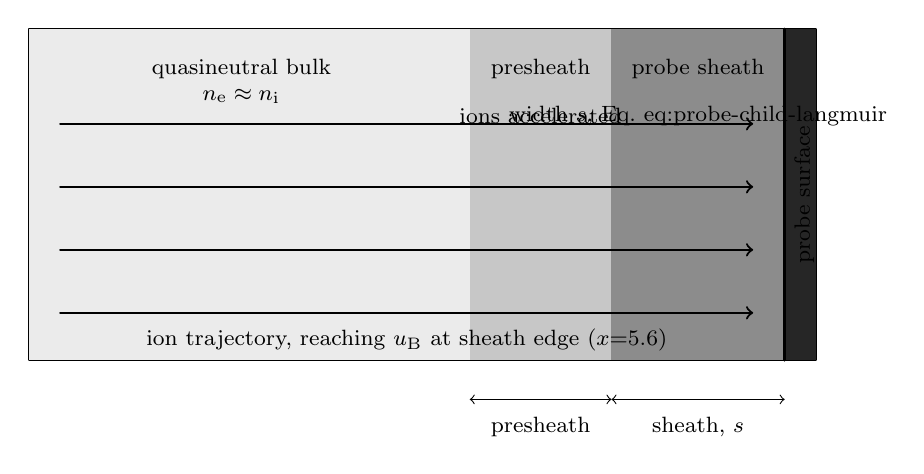
\begin{tikzpicture}[x=1cm,y=1cm,line cap=round,line join=round]

 \draw[thick] (0,0) rectangle (10,4.2);

 \fill[black!8] (0,0) rectangle (5.6,4.2);
 \fill[black!22] (5.6,0) rectangle (7.4,4.2);
 \fill[black!45] (7.4,0) rectangle (9.6,4.2);
 \fill[black!85] (9.6,0) rectangle (10,4.2);

 \draw[very thick] (9.6,0) -- (9.6,4.2);

 \node at (2.7,3.7) {\footnotesize quasineutral bulk};
 \node at (2.7,3.35) {\footnotesize $n_{\mathrm{e}} \approx n_{\mathrm{i}}$};

 \node at (6.5,3.7) {\footnotesize presheath};
 \node[align=center] at (6.5,3.1) {\footnotesize ions accelerated};

 \node at (8.5,3.7) {\footnotesize probe sheath};
 \node[align=center] at (8.5,3.1) {\footnotesize width $s$, Eq.~\eqref{eq:probe-child-langmuir}};

 \node[rotate=90] at (9.85,2.1) {\footnotesize probe surface};

 \foreach \y in {0.6,1.4,2.2,3.0}{
 \draw[->,thick] (0.4,\y) -- (9.2,\y);
 }
 \node at (4.8,0.25) {\footnotesize ion trajectory, reaching $u_{\mathrm{B}}$ at sheath edge ($x{=}5.6$)};

 \draw[<->] (5.6,-0.5) -- (7.4,-0.5);
 \node at (6.5,-0.85) {\footnotesize presheath};
 \draw[<->] (7.4,-0.5) -- (9.6,-0.5);
 \node at (8.5,-0.85) {\footnotesize sheath, $s$};

\end{tikzpicture}
\caption{Schematic cross-section of the presheath and sheath adjacent to a negatively biased planar probe surface. Shading darkens toward the probe surface, indicating progressive departure from quasineutrality; ion trajectories (arrows) accelerate through the presheath and cross the sheath edge at approximately the Bohm velocity $u_{\mathrm{B}}$. No experimental data are represented; the figure is a conceptual aid only.}
\label{fig:probe-sheath-schematic}
\end{figure}

\subsection{Sheath Expansion, Effective Collection Area, and Orbit-Limited Collection}

A subtlety with direct consequences for density extraction: the probe's effective collecting area is not, in general, its physical geometric area, because the sheath boundary expands outward as bias is driven more negative, per Equation~\eqref{eq:probe-child-langmuir}. For a planar probe this is often small; but for the cylindrical or spherical tips used in most laboratory probes, sheath expansion increases the effective collecting area with bias, producing an ion-saturation branch that fails to saturate cleanly, a departure from the idealized flat saturation implicit in Equation~\eqref{eq:probe-Iis}. When the probe radius is comparable to or smaller than the sheath thickness, ion collection is better described by orbital-motion-limited (OML) theory, in which ions with sufficient angular momentum are deflected around the probe without being collected; the choice among planar, cylindrical, and OML collection models is itself a nontrivial source of uncertainty in the inferred density.

\subsection{Global Perturbation of the Bulk Plasma}

Beyond the local sheath, the probe perturbs the plasma non-locally: any current it draws must be returned through some other conducting surface, whether the chamber wall or a partner tip; this return current modifies the ambipolar balance near both the probe and its return path, significant when the probe occupies a non-negligible fraction of the plasma volume or draws electron-saturation current comparable to the discharge current. In small or low-power sources this is not a second-order correction: gyrofluid-simulation-based studies show the collected current is sensitive to the assumed background temperature profile in ways a purely local, unperturbed-plasma interpretation cannot capture \cite{ref0194}.

\section{Survival, Contamination, and Erosion in High-Flux Environments}
\label{sec:probes-survival}

\subsection{Thermal and Sputtering Loads}

The very high-flux, high-energy environments where ion energy flux quantification is most urgently needed, magnetized fusion edge and divertor plasmas, high-power-density processing reactors, and thruster plumes, are also the environments most hostile to a solid probe tip. A probe surface immersed there is subject simultaneously to Joule heating from the collected current, kinetic heating from ion bombardment, and physical sputtering that erodes the surface and alters its geometry over a single sweep or campaign. Because the ion energy delivered to the probe is set by the same sheath acceleration this monograph seeks to quantify, a probe deployed to measure high ion energy flux is unavoidably subjected to that flux as a material load, forcing rapid sweeps and tight duty-cycling so cumulative damage does not compromise tip geometry within a single measurement.

\subsection{Contamination and Its Effect on the Collected Characteristic}

A second, subtler failure mode is surface contamination: deposition of sputtered material, condensable reaction products, or dielectric films, which changes the effective work function and, in the worst case, forms a partially insulating layer that rectifies the collected current asymmetrically between bias polarities. A contaminated probe can produce an I-V trace that appears smooth and reasonable while yielding a systematically biased $T_{\mathrm{e}}$ or $n_{\mathrm{e}}$, since Equation~\eqref{eq:probe-exp-region} implicitly assumes a work function and secondary-electron yield constant across the sweep and known a priori. This is acute in laser-produced and ablation plasmas, where ablated material can coat the tip between shots, necessitating frequent conditioning or replacement. In reactive or dusty discharges, similar concerns motivate cross-validation of probe-derived $T_{\mathrm{e}}$ and $n_{\mathrm{e}}$ against independent, non-contact techniques (Section~\ref{sec:probes-alternatives}).

\subsection{Duty-Cycled and Transient Operation}

Where continuous exposure is impractical, probes are duty-cycled: inserted briefly into the high-flux region, swept, and withdrawn before cumulative erosion or thermal loading becomes significant, or operated only during a single transient pulse. Triple-probe systems, requiring no sweep, suit this mode particularly well. In all such cases, the diagnostic strategy is fundamentally a compromise between the resolution demanded by the physics and the survivability of the sensor, a compromise that becomes less favorable as ion energy flux increases, precisely the regime of greatest interest here.

\section{Interpretation Ambiguities in Non-Maxwellian and Magnetized Plasmas}
\label{sec:probes-ambiguities}

\subsection{Departures from a Maxwellian Electron Energy Distribution}

The entire derivation in Section~\ref{sec:probes-langmuir-theory}, from Equation~\eqref{eq:probe-exp-region} to the slope-based extraction of $T_{\mathrm{e}}$ in Equation~\eqref{eq:probe-Te-slope}, rests on the assumption that the electron population feeding the probe sheath is locally Maxwellian. This fails routinely in low-pressure, non-equilibrium discharges, where the electron energy distribution commonly exhibits a bi-Maxwellian structure (a cold bulk plus a hotter tail sustained by discharge heating), a depleted high-energy tail, or a power-law kappa tail more familiar from space plasmas. When the true distribution is non-Maxwellian, a single-slope fit to $\ln I_{\mathrm{e}}(V)$ no longer yields a well-defined temperature: the slope varies with bias, and the reported "electron temperature" depends on the fit window, an ambiguity with no general resolution short of recovering the full distribution. The more rigorous alternative is the Druyvesteyn method, inverting the distribution directly from the second derivative of the retarded current,
\begin{equation}
f_{\mathrm{e}}(E) \;\propto\; \sqrt{E}\; \frac{\mathrm{d}^2 I_{\mathrm{e}}}{\mathrm{d}V^2}, \qquad E = e\left(\phi_{\mathrm{p}} - V\right),
\label{eq:druyvesteyn}
\end{equation}
at the cost of extreme noise sensitivity, since numerical second differentiation amplifies high-frequency noise in the raw trace. Joint measurements of the electron energy distribution, plasma potential, and density from a single trace in tokamak edge plasma demonstrate both the payoff of extracting the full distribution and the added complexity this requires relative to a simple two-parameter Maxwellian fit \cite{ref0213}.

\subsection{Fluctuation-Induced Bias}

A related, underappreciated source of error arises when plasma parameters fluctuate on timescales comparable to or shorter than the sweep time. Because Equation~\eqref{eq:probe-exp-region} is nonlinear in both $T_{\mathrm{e}}$ and $\phi_{\mathrm{p}}$, a time-averaged I-V trace acquired during a fluctuating plasma does not, in general, correspond to the time-averaged parameters; Jensen's inequality guarantees that averaging a convex function of a fluctuating quantity biases the result relative to evaluating that function at the mean. This is especially acute in scrape-off-layer turbulence studies, where probes resolve correlation lengths of intermittent structures, and where fluctuation statistics measured across devices such as Alcator C-Mod provide a benchmark against which probe-inferred correlation lengths must be interpreted with this bias in mind \cite{ref0611}.

\subsection{Magnetized Plasmas and Anisotropic Collection}

A strong background magnetic field introduces a further, qualitatively distinct difficulty: charged-particle collection becomes intrinsically anisotropic, since electrons and ions gyrate about field lines with gyroradii comparable to, larger than, or smaller than the probe dimension and sheath thickness. When the electron gyroradius is small compared with the probe and sheath, collection along the field is strongly enhanced relative to collection across field lines, and the isotropic expression underlying Equation~\eqref{eq:probe-Ies} must be replaced by an angle- and field-dependent model; probe orientation relative to $\mathbf{B}$ becomes an experimental variable itself. At the sheath itself, an oblique field modifies the ion acceleration and effective Bohm criterion relative to the unmagnetized case (Section~\ref{sec:probes-sheath-perturbation}), so a model calibrated against unmagnetized theory can misattribute magnetic effects to spurious changes in $T_{\mathrm{e}}$ or $n_{\mathrm{e}}$.

\subsection{Collisional and Orbit-Limited Corrections}

Even absent a magnetic field, the idealized collisionless, planar sheath model underlying Equations~\eqref{eq:probe-exp-region}--\eqref{eq:probe-child-langmuir} can fail once the sheath or presheath thickness becomes comparable to the ion- or electron-neutral mean free path, a regime found in higher-pressure processing plasmas and dense, partially ionized sources. Collisions randomize ion trajectories that would otherwise cross ballistically, softening the sharp saturation predicted by orbit-limited or Child-Langmuir theory and adding the mean free path as an extra free parameter. Comparative studies across multiple probe configurations under identical conditions are needed to isolate genuine physics from artifacts of the collection-theory assumptions; no single analytic probe theory can be trusted in isolation.

\section{The Case for Non-Intrusive Alternatives}
\label{sec:probes-alternatives}

The preceding sections establish a consistent pattern: every strength of the Langmuir probe and its derivatives, direct current collection, simple theory, high resolution, is coupled to an equally direct vulnerability, because the measurement mechanism is inseparable from the physical presence of a biased electrode in the plasma. The probe sheath perturbs the local ambipolar balance (Section~\ref{sec:probes-sheath-perturbation}); the probe surface is degraded by the same high-energy ion flux it is deployed to measure (Section~\ref{sec:probes-survival}); and the interpretation of the collected current becomes ambiguous precisely in the non-Maxwellian, magnetized, and collisional regimes that characterize many plasmas of greatest interest (Section~\ref{sec:probes-ambiguities}). None of these is a matter of instrumental refinement that further engineering can eliminate; they follow from the fact that probe theory presupposes a well-characterized sheath and electron distribution, exactly the quantities least certain under the most demanding conditions.

This has motivated a sustained effort to cross-validate, and where possible replace, electrostatic probe measurements with diagnostics that do not require inserting a material object into the plasma. Optical techniques that infer $T_{\mathrm{e}}$ and $n_{\mathrm{e}}$ from the plasma's own radiated or scattered light are the most direct alternative, and a substantial body of work has benchmarked these methods against Langmuir probes under matched conditions, with discrepancies traceable to exactly the perturbation and non-Maxwellian effects discussed above \cite{ref0237}. Comparable cross-validation between Langmuir probes and laser Thomson scattering, which infers $T_{\mathrm{e}}$ and $n_{\mathrm{e}}$ from the Doppler-broadened spectrum of light scattered incoherently from free electrons without any sheath assumption, has been carried out in Hall-effect plasma sources, a regime combining high power density with strong non-uniformity in which probe survivability and interpretation are both challenged \cite{ref0355}. Broader comparisons reinforce the finding that the two techniques agree well in benign, near-Maxwellian, weakly perturbed plasmas but diverge as conditions approach the regimes identified in Section~\ref{sec:probes-ambiguities} \cite{ref0354}, and foundational treatments of Thomson-scattering theory establish the conditions under which the scattered spectrum can be inverted for $n_{\mathrm{e}}$ and $T_{\mathrm{e}}$ without the sheath-based assumptions underlying every probe method in this chapter \cite{ref0384}.

Taken together, this literature supports two conclusions motivating the remainder of this monograph. First, electrostatic probes and RFEAs remain indispensable where their limitations are well characterized and the operating regime is benign: low-flux, weakly magnetized, near-Maxwellian plasmas at modest density, where the sheath model of Section~\ref{sec:probes-sheath-perturbation} is trustworthy and the probe survives long enough to complete a measurement. Second, and more important here, the plasmas of greatest practical interest, those with high ion energy flux across the sheath, are systematically the plasmas in which intrusive measurements are least reliable, because high flux threatens probe survival, drives the sheath and presheath into regimes where simple collection theory breaks down, and is often associated with non-Maxwellian or magnetized conditions. This inverse relationship between measurement difficulty and diagnostic reliability establishes the case, developed in the chapters that follow, for characterizing ion energy flux without placing a solid, current-collecting object into the sheath being measured.

\section{Summary}
\label{sec:probes-summary}

This chapter developed the theoretical basis of electrostatic probe diagnostics, from the exponential I-V characteristic and its use in extracting $T_{\mathrm{e}}$, $n_{\mathrm{e}}$, and $\phi_{\mathrm{p}}$ (Section~\ref{sec:probes-langmuir-theory}), through the principal probe geometries and the RFEA used to reconstruct $f_{\mathrm{i}}(v)$ and $\Gamma_{E}$ directly (Section~\ref{sec:probes-variants}). It then examined the sheath that inevitably forms around any biased probe surface, its Child-Langmuir scaling, and the resulting local and global perturbation of the measured plasma (Section~\ref{sec:probes-sheath-perturbation}), before turning to high-flux operation, where thermal loading, sputtering erosion, and contamination progressively degrade fidelity and threaten survival (Section~\ref{sec:probes-survival}). The chapter's central difficulty, developed in Section~\ref{sec:probes-ambiguities}, is that the interpretive framework underlying every probe method presupposes a Maxwellian, unmagnetized, collisionless plasma, an assumption that fails precisely in the non-equilibrium, magnetized, collisional regimes most relevant to modern plasma technology and fusion-edge research. The comparative evidence in Section~\ref{sec:probes-alternatives}, drawn from benchmarking against optical and Thomson-scattering techniques, shows these limitations to be structural rather than instrumental, growing most severe exactly where $\Gamma_E$ is largest, setting the stage for the non-intrusive diagnostic strategies developed in the chapters that follow.
